%----------------------------------------------------------------------------
\section{A szerkesztéshez használatos, Windows alapú eszközök}
%----------------------------------------------------------------------------
Ez a sablon Windows operációs rendszer alatt készült TeXnicCenter 1 Beta 7.01 szerkesztővel. A TeXnicCenter egy \LaTeX-szerkesztőprogram számtalan hasznos -- és ráadásul jól működő -- szolgáltatással (\figref{TexnicCenter} ábra). A szoftver ingyenesen letölthető a\\\url{http://www.texniccenter.org/} címről.

\begin{figure}[!ht]
\centering
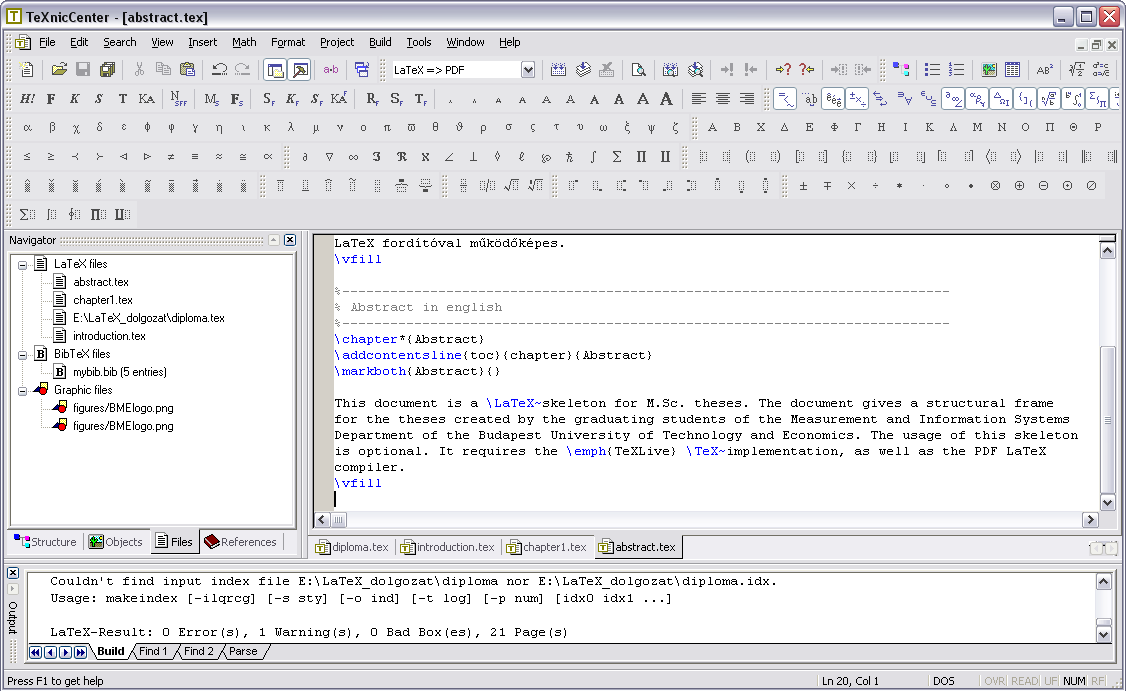
\includegraphics[width=150mm, keepaspectratio]{figures/TeXnicCenter.png}
\caption{A TeXnicCenter Windows alapú \LaTeX-szerkesztő.} 
\label{fig:TexnicCenter}
\end{figure}

Egy másik használható Windows alapú szerkesztőprogram a LEd (LaTeX Editor,\\\url{http://www.latexeditor.org/}), a TeXnicCenter azonban stabilabb, gyorsabb, és jobban használható.
